\documentclass[xetex,mathserif,serif]{beamer}
\usepackage{polyglossia}
\setdefaultlanguage[babelshorthands=true]{russian}
\usepackage{minted}
\usepackage{tabu}

\useoutertheme{infolines}

\usepackage{fontspec}
\setmainfont{FreeSans}
\newfontfamily{\russianfonttt}{FreeSans}

\setbeamertemplate{blocks}[rounded][shadow=false]

\setbeamercolor*{block title alerted}{fg=red!50!black,bg=red!20}
\setbeamercolor*{block body alerted}{fg=black,bg=red!10}

\tabulinesep=1.2mm

\title{Многопоточное программирование}
\subtitle{Часть 2: низкоуровневая многопоточность}
\author[Юрий Литвинов]{Юрий Литвинов\\\small{\textcolor{gray}{yurii.litvinov@gmail.com}}}
\date{9}

\newcommand{\todo}[1] {
	\begin{center}\textcolor{red}{TODO: #1}\end{center}
}

\newcommand{\DownArrow} {
	\hspace{2cm}\begin{LARGE}$\downarrow$\end{LARGE}
}

\begin{document}

	\frame{\titlepage}

	\section{Введение}

	\begin{frame}
		\frametitle{Примитивы синхронизации}
		\begin{itemize}
			\item Лучше необходимости синхронизации вообще избегать
			\item Бывают:
			\begin{itemize}
				\item User-mode --- атомарные операции, реализующиеся на процессоре и не требующие участия планировщика
				\item Kernel-mode --- примитивы, управляющие тем, как поток обрабатывается планировщиком
				\begin{itemize}
					\item Более тяжеловесные и медленные (до 1000 раз по сравнению с ``без синхронизации вообще'')
					\item Позволяют синхронизировать даже разные процессы
				\end{itemize}
			\end{itemize}
		\end{itemize}
	\end{frame}

	\section{User-mode-синхронизация}

	\begin{frame}
		\frametitle{Атомарные операции}
		\begin{itemize}
			\item Чтения и записи следующих типов всегда атомарны: Boolean, Char, (S)Byte, (U)Int16, (U)Int32, (U)IntPtr, Single, ссылочные типы
			\item \mintinline{csharp}|Volatile|
			\begin{itemize}
				\item \mintinline{csharp}|Volatile.Write|
				\item \mintinline{csharp}|Volatile.Read|
				\item Связано с понятием Memory Fence, требует синхронизации ядер
				\item Есть ключевое слово \mintinline{csharp}|volatile|: \mintinline{csharp}|private volatile int flag = 0;|
				\item \mintinline{csharp}|Volatile.Write| должен быть последней операцией записи, \mintinline{csharp}|Volatile.Read| --- первой операцией чтения
			\end{itemize}
		\end{itemize}
	\end{frame}

	\begin{frame}[fragile]
		\frametitle{Пример}
		\begin{minted}{csharp}
private int flag = 0;
private int value = 0;

public void Thread1() {
    value = 5;
    Volatile.Write(ref flag, 1);
}

public void Thread2() {
    if (Volatile.Read(ref flag) == 1)
        Console.WriteLine(value);
}
		\end{minted}
	\end{frame}

	\begin{frame}
		\frametitle{Interlocked}
		\begin{itemize}
			\item Одновременные чтение и запись в одной ``транзакции''
			\begin{itemize}
				\item \mintinline{csharp}|public static Int32 Increment(ref Int32 location);|
				\item \mintinline{csharp}|public static Int32 Decrement(ref Int32 location);|
				\item \mintinline{csharp}|public static Int32 Add(ref Int32 location, Int32 value);|
				\item \mintinline{csharp}|public static Int32 Exchange(ref Int32 location, Int32 value);|
				\item \mintinline{csharp}|public static Int32 CompareExchange(ref Int32 location, |
					\mintinline{csharp}| Int32 value, Int32 comparand);|
			\end{itemize}
		\end{itemize}
	\end{frame}

	\begin{frame}[fragile]
		\frametitle{Interlocked lock-free-операции}
		\framesubtitle{Compare-And-Swap loop}
		\begin{footnotesize}
			\begin{minted}{csharp}
public static Int32 Maximum(ref Int32 target, Int32 value) {
    Int32 currentVal = target, startVal = 0, desiredVal = 0;
    do {
        startVal = currentVal;
        desiredVal = Math.Max(startVal, value);
        // Тут другой поток мог уже испортить target, так что если она изменилась,
        // надо начать всё сначала.
        currentVal = Interlocked.CompareExchange(ref target, desiredVal, startVal);
    } while (startVal != currentVal);
    return desiredVal;
}
			\end{minted}
		\end{footnotesize}
	\end{frame}

	\begin{frame}[fragile]
		\frametitle{Крутящееся ожидание}
		\begin{small}
			\begin{minted}{csharp}
internal struct SimpleSpinLock {
    private int resourceInUse;

    public void Enter() {
        while (true) {
            if (Interlocked.Exchange(ref resourceInUse, 1) == 0) 
                return;
        }
    }

    public void Leave() {
        Volatile.Write(ref resourceInUse, 0);
    }
}
			\end{minted}
			Считается антипаттерном, но в некоторых ситуациях лучше lock-ов
		\end{small}
	\end{frame}

	\begin{frame}
		\frametitle{Управление планировщиком}
		\begin{small}
			\begin{itemize}
				\item \mintinline{csharp}|Thread.Sleep(0)| --- ничего не делает, если остальные готовые потоки меньше приоритетом
				\item \mintinline{csharp}|Thread.Sleep(1)| --- отдаёт управление потоку, даже если его приоритет меньше
				\item \mintinline{csharp}|Thread.Yield()| --- нечто среднее (не вызовет переключения потоков, если желающих нет, в отличие от \mintinline{csharp}|Thread.Sleep(1)|, но отдаст ядро потоку с меньшим приоритетом)
				\item \mintinline{csharp}|Thread.SpinWait| --- просьба процессору с гипертредингом отдать ядро
				\item Очередной способ прострелить себе ногу --- инверсия приоритетов
				\begin{itemize}
					\item Поток с низким приоритетом захватил ресурс, нужный потоку с высоким приоритетом
					\item Поток с высоким приоритетом крутится в ожидании, никогда не отдавая управление потоку, который мог бы отдать ресурс (livelock)
				\end{itemize}
			\end{itemize}
		\end{small}
	\end{frame}

	\section{Kernel-mode-синхронизация}

	\begin{frame}
		\frametitle{Примитивы уровня ядра ОС}
		\begin{itemize}
			\item \mintinline{csharp}|WaitHandle| --- всё, что можно ожидать
			\begin{itemize}
				\item \mintinline{csharp}|EventWaitHandle|
				\begin{itemize}
					\item \mintinline{csharp}|AutoResetEvent| --- по сути, булевый флаг, поддерживаемый ОС
					\item \mintinline{csharp}|ManualResetEvent| --- тоже булевый флаг, но сбрасывается вручную
				\end{itemize}
				\item Semaphore --- целое число, поддерживаемое ОС
				\item Mutex --- семафор, пропускающий только один поток
			\end{itemize}
		\end{itemize}
	\end{frame}

	\begin{frame}[fragile]
		\frametitle{Пример (замок на Event-ах)}
		\begin{small}
			\begin{minted}{csharp}
internal sealed class SimpleWaitLock : IDisposable {
    private readonly AutoResetEvent available;
    public SimpleWaitLock() {
        available = new AutoResetEvent(true); 
    }

    public void Enter() {
        available.WaitOne();
    }

    public void Leave() {
        available.Set();
    }

    public void Dispose() { available.Dispose(); }
}
			\end{minted}
		\end{small}
	\end{frame}

	\begin{frame}[fragile]
		\frametitle{Пример (замок на семафорах)}
		\begin{small}
			\begin{minted}{csharp}
public sealed class SimpleWaitLock : IDisposable {
    private readonly Semaphore available;
    public SimpleWaitLock(Int32 maxConcurrent) {
        available = new Semaphore(maxConcurrent, maxConcurrent);
    }

    public void Enter() {
        available.WaitOne();
    }

    public void Leave() {
        available.Release(1);
    }

    public void Dispose() { available.Close(); }
}
			\end{minted}
		\end{small}
	\end{frame}

	\begin{frame}[fragile]
		\frametitle{Пример (мьютекс, он сам замок)}
		\begin{small}
			\begin{minted}{csharp}
internal class SomeClass : IDisposable {
    private readonly Mutex aLock = new Mutex();

    public void Method1() {
        aLock.WaitOne();
        Method2();  // Тут рекурсивный захват мьютекса
        aLock.ReleaseMutex();
    }

    public void Method2() {
        aLock.WaitOne();
        ...
        aLock.ReleaseMutex();
    }

    public void Dispose() { aLock.Dispose(); }
}
			\end{minted}
		\end{small}
	\end{frame}

	\begin{frame}
		\frametitle{Гибридные конструкции}
		\begin{itemize}
			\item \mintinline{csharp}|ManualResetEventSlim|
			\item \mintinline{csharp}|SemaphoreSlim|
			\item \mintinline{csharp}|ReaderWriterLockSlim|
			\item \mintinline{csharp}|Monitor|
			\begin{itemize}
				\item Ключевое слово \mintinline{csharp}|lock|
			\end{itemize}
		\end{itemize}
	\end{frame}

	\begin{frame}[fragile]
		\frametitle{Пример}
		\begin{footnotesize}
			\begin{minted}{csharp}
internal sealed class Transaction {
    private readonly Object aLock = new Object(); 
    private DateTime timeOfLastTrans;

    public void PerformTransaction() {
        Monitor.Enter(aLock);
        timeOfLastTrans = DateTime.Now;
        Monitor.Exit(aLock);
    }

    public DateTime LastTransaction {
        get { 
            Monitor.Enter(aLock); 
            DateTime temp = timeOfLastTrans;
            Monitor.Exit(aLock); 
            return temp;
        }
    }
}
			\end{minted}
		\end{footnotesize}
	\end{frame}

	\begin{frame}[fragile]
		\frametitle{lock}
		\begin{small}
			\begin{minted}{csharp}
private void SomeMethod() {
    lock (this) {
        ...
    }
}
			\end{minted}
			Так писать нельзя: любой, кто имеет ссылку на this, может взять на него замок без его ведома, что может привести к дедлоку, если замок взят из другого потока. Правильнее:
			\begin{minted}{csharp}
private Object lockObject = new Object();

private void SomeMethod() {
    lock (lockObject) {
        ...
    }
}
			\end{minted}
		\end{small}
	\end{frame}

	\begin{frame}
		\frametitle{Литература}
		\framesubtitle{Must read}
		\begin{columns}
			\begin{column}{0.6\textwidth}
				Jeffrey Richter, CLR via C\# (4th Edition), Microsoft Press, 2012. 894pp.
				\vspace{3cm}
			\end{column}
			\begin{column}{0.3\textwidth}
				\begin{center}
					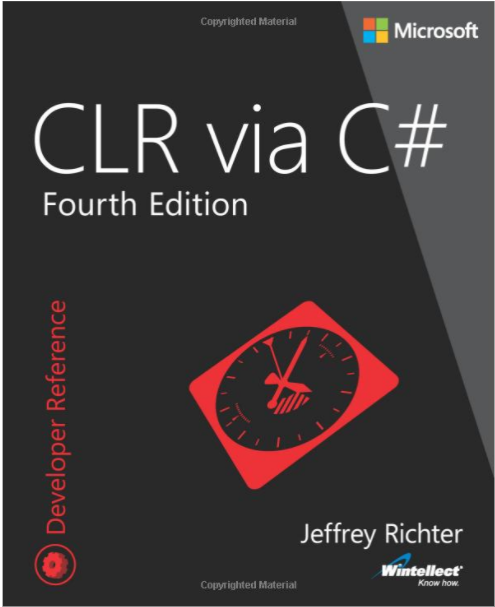
\includegraphics[width=\textwidth]{clrViaCSharpCover.png}
				\end{center}
			\end{column}
		\end{columns}
	\end{frame}

\end{document}
